This chapter presents the methodologies and tools used to implement the end-to-end pipeline for synthetic image generation and object detection model training. The first three sections introduce the overall workflow, scoping, and used datasets of the work. After that, the implementation of the pipeline is described. The implementation is divided into three main parts: LoRA training, synthetic image generation, and object detection model training. Figure \ref{fig:phaises} shows how the custom LoRA model is trained, how it is integrated into the SDXL base model to generate synthetic images, and how the generated images are processed for object detection model training.


\begin{figure}[!ht]
    \centering
    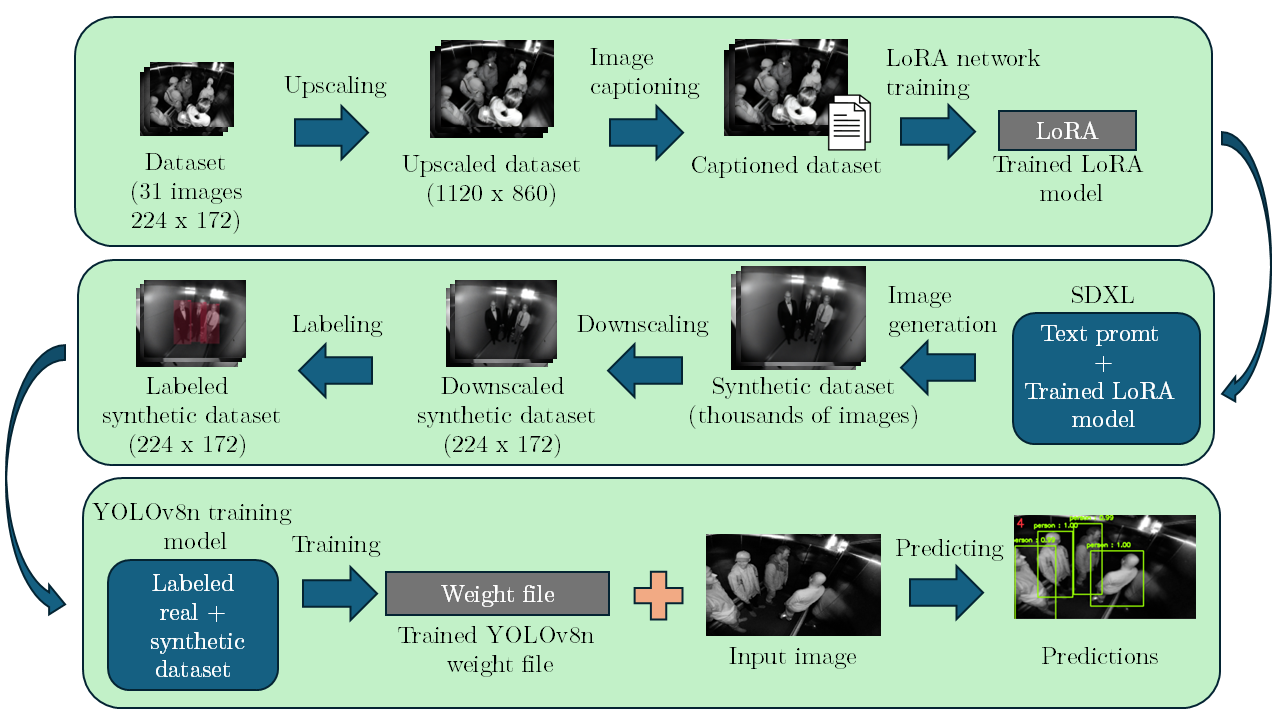
\includegraphics[width=1\textwidth]{images/vaiheet.png}
    \caption{Overview of the synthetic image generation and object detection training workflow.}
   \label{fig:phaises}
\end{figure}

The first row of Figure~\ref{fig:phaises} illustrates the preparation of the dataset for LoRA training. The process begins by selecting 31 different images captured from near-infrared (NIR) sensor, which are then upscaled using Upscayl from 224 x 172 to 1120 x 860 pixels, as the pretrained SDXL model requires high-resolution images for training. The upscaled images are captioned using Taggui for efficient captioning. The captioned dataset are used to train the LoRA model with Kohya-ss.

The second row shows how the pretrained SDXL base model is fine-tuned by interating the trained LoRA to generate synthetic images resembling those captured by the NIR sensor. The generation process is performed using Stable Diffusion WebUI Forge. Approximately 4000 images were initially generated, after which the synthetic dataset was cleaned to 2500 images. The cleaned dataset was downscaled to match the original sensor image resolution and then annotated together with sensor images using Darkmark for YOLOv8n model training. From the annotated data there was created 23 different training datasets with varying combinations of real and synthetic images.

The last row represents the training phase of 23 YOLOv8n models, each fine-tuned using one of the dataset variations. The training was performed using the Ultralytics Python library. The final outcome consists of 23 fine-tuned YOLOv8n models capable of detecting people in NIR images


\section{Workflow}
\label{sec:workflow}
The development of the object detection model follows generally the same steps as machine learning workflows. Typically these workflows are divided into five main categories: scoping, data management, model development, verification, and deployment. These categories, along with their associated phases and example tasks, are listed in Table~\ref{tab:ml_workflow_grouped}.

In the following sections scoping and data management phases are described in Sections~\ref{sec:scoping} and \ref{sec:data_management}. Model development for synthetic image generation is presented in Section~\ref{sec:lora}, and object detection model training is detailed in Section~\ref{sec:object_detection_training}. Verification is implemented in Chapter~\ref{ch:results} to evaluate the object detection models. The deployment phase is not covered in this work, as the focus is on evaluating the effect of synthetic images on object detection model performance.

\begin{table}[!p]
    \caption{Overview of the basic machine learning workflow grouped by categories and phases, with example tasks \cite{workflownumerical, crispmlq, Paleyes_2022}.}
\label{tab:ml_workflow_grouped}
\def\arraystretch{1.5}
\begin{NiceTabular}{>{\centering\arraybackslash}m{0.18\textwidth} >{\centering\arraybackslash}m{0.22\textwidth} m{0.50\textwidth}}[hvlines]
\textbf{Workflow Category} & \textbf{Workflow Phase} & \multicolumn{1}{c}{\textbf{Example Tasks}} \\
\Block{2-1}{Scoping}
    & Problem Identification & Defining the problem, defining requirements and constraints, conducting literature review on similar problems \\
    & Objectives and Resources & Setting project goals, determining data requirements, examining available tools, models, and other resources \\
\Block{2-1}{Data Management}
    & Data Collection & Discovering existing data, recording new data \\
    & Data Preparation & Annotating, cleaning, transforming, reducing, and augmenting data; generating synthetic data; splitting data into training, validation, and testing sets \\
\Block{2-1}{Model Development}
    & Model Selection & Choosing model architecture based on requirements, Selecting pretrained model for fine-tuning or fully training new model from scratch \\
    & Model Training & Configuring hyperparameters and training the model \\
\Block{2-1}{Verification}
    & Model Evaluation & Calculating evaluation metrics, comparing results against criteria, iteratively tuning data and model as needed \\
    & Test-based Verification & Performing real-world testing or simulated tests, evaluating model on production hardware \\
\Block{2-1}{Deployment}
    & Model Deployment & Exporting and integrating the model into applications, deploying to edge devices or cloud infrastructure \\
    & Monitoring & Tracking model performance, updating the model with new data, retraining as required \\
\end{NiceTabular}
\end{table}


\section{Scoping}
\label{sec:scoping}

The central question addressed in this work is whether synthetic data can be used to improve the performance of an object detection model. To answer this question, three main goals were defined:
\begin{enumerate}

    \item Review existing methods for generating synthetic images and their effectiveness in improving object detection model performance. Based on this review, one approach is selected for implementation: a diffusion-based text-to-image model.

    \item Implement a complete synthetic data generation and object detection pipeline from scratch.

    \item Analyse the effect of different combinations of real and synthetic data on object detection model performance.

\end{enumerate}


The object detection task in this work focuses on detecting people in images captured by a Near-Infrared (NIR) sensor in small indoor environments. This domain was chosen because preliminary tests with the YOLOv8n base model showed that people could be detected reasonably well, yet there remained significant room for improvement. This makes it a suitable and challenging test case for exploring the potential of synthetic data augmentation in object detection.

The following requirements and constraints were defined for this work:

\begin{itemize}

    \item The implementation must use only open-source tools and models.

    \item The text-to-image model must generate images that closely resemble the characteristics of real NIR sensor images.

    \item The text-to-image generation process must be automated to produce images across varied scenarios.

    \item The object detection model must be trained with hyperparameters that improve performance compared to the base model trained with real images only.

    \item Multiple object detection models must be trained with different combinations of real and synthetic images to analyse their effect on model performance.

    \item The best-performing object detection model's confidence threshold must be optimized to achieve the highest possible F1-score.

\end{itemize}

This work adopts the concept of \textit{data-centric AI} as its conceptual framework for training the object detection model. Data-centric AI focuses on improving model performance primarily through refining and expanding the training dataset, while keeping the model architecture and hyperparameters largely unchanged \cite{data_centric_ai_survey}. In this work, this approach is applied by maintaining consistent hyperparameters for the object detection model as long as the results meet the defined requirements. The framework also supports the core idea of evaluating the effect of synthetic data by training multiple object detection models with different combinations of real and synthetic images.

Table~\ref{tab:used_tools} lists the tools and models used in this work, along with the motivation for their selection. All tools and models meet the requirement of being open-source, ensuring accessibility and reproducibility of the research.

\begin{table}[!h]
        \caption{Tools used in the workflow and motivation for their selection.}
    \label{tab:used_tools}
    \centering
    \begin{tabular}{|p{0.18\textwidth}|p{0.18\textwidth}|p{0.45\textwidth}|}
    \hline
    \textbf{Task} & \textbf{Tool/Model} & \textbf{Motivation for choice} \\ \hline \hline
    Upscaling & Upscayl \cite{upscayl} & Upscaling and enhancing multiple images to the desired resolution \\
    \hline
    Captioning & Taggui \cite{taggui} & Enables fast captioning of multiple images.\\
    \hline
    Text-to-image model & SDXL \cite{sdxlbase} &  Open-source, high-performance, and flexible diffusion model suitable for fine-tuning.\\
    \hline
    LoRA training & Kohya SS \cite{kohya-ss} & Provides a user-friendly interface for LoRA training. \\
    \hline
    Text-to-image generation & Stable Diffusion WebUI Forge \cite{stable-diffusion-webui-forge} & User-friendly interface for Stable Diffusion-based image generation; includes useful automation extensions for generating diverse image scenarios. \\
    \hline
    Annotation & Darkmark \cite{darkmark} & Efficient annotation tool with built-in analytics for annotation quality control. \\
    \hline
    Object detection model & YOLOv8n \cite{yolov8} & Lightweight and fast object detector, widely used in object detection studies. \\
    \hline
    Object detection model training & Ultralytics \cite{ultralytics} & Python library for YOLO models providing extensive functionality for training and evaluation. \\
    \hline
    \end{tabular}
\end{table}



 %From the literature research in section \ref{sec:synthetic_data_object_detection}, it was found that there is not much research about generating synthetic images from text-to-image models. Also, some of those studies generated images that do not seem to match the characteristics of real images, as in paper \cite{REUTOV2023335}, which gives motivation to research this topic further.

\section{Data Management}
\label{sec:data_management}
The initial dataset consists of near-infrared (NIR) images recorded inside elevators. These recordings were obtained from a student project dataset for reflection recognition research, where videos were captured in elevators using an NIR sensor. Additional recordings were collected with the same sensor to increase dataset diversity for training and testing. The recordings were taken from a tilted top-view perspective across elevators with varying backgrounds, lighting conditions, and occupancy. Since the focus of this work is on people detection, the dataset includes various human-related scenarios, such as individuals standing very close to the sensor or lying on the floor. Example images from the dataset are shown in Figure~\ref{fig:testing}.

\begin{figure}[!h]
    \centering
    \subcaptionbox{}{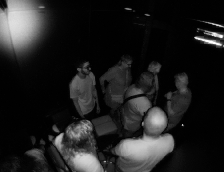
\includegraphics[height=9\baselineskip]{images/methotologies/Dataset/testing/royale_20240710_110908_frame180.png}} \quad
    \subcaptionbox{}{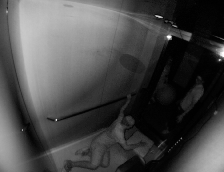
\includegraphics[height=9\baselineskip]{images/methotologies/Dataset/testing/royale_20240710_113404_frame336.png}} \quad
    \subcaptionbox{}{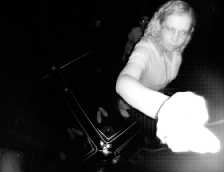
\includegraphics[height=9\baselineskip]{images/methotologies/Dataset/testing/royale_20240710_134224_frame1146.png}} \quad
    \subcaptionbox{}{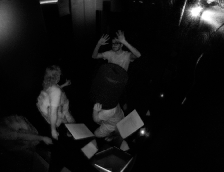
\includegraphics[height=9\baselineskip]{images/methotologies/Dataset/testing/royale_20240710_141816_frame366.png}} \quad
    \caption{Example images from the NIR sensor: (a) crowded elevator, (b) person lying on the floor, (c) person very close to the sensor, (d) various objects and obscured people.}
    \label{fig:testing}
\end{figure}

Captured images have a resolution of 224 x 172 pixels and are 1-channel grayscale. Since most tools used in this work require 3-channel images, each image was converted to RGB by replicating the grayscale values across all channels.
The dataset was improved by removing adjacent frames of the recordings to prevent redundancy. Frames containing reflections from mirrors or reflective surfaces were removed, as they could cause false positive detections. Reflection detection itself was scoped out for future research.

After preprocessing, the dataset contained 1598 images for object detection (568 training, 284 validation, 746 testing) and 31 images for LoRA training. Additionally, 2500 synthetic images were later generated for object detection model training.

\section{Synthetic Image Generation}
\label{sec:lora}
\subsection{Upscaling}
The SDXL base model is trained with high-resolution images of varying aspect ratios, close to a pixel count of 1024 x 1024  \cite{podell2023sdxlimprovinglatentdiffusion}. To ensure compatibility with the base model, the LoRA should also be trained on images of similar resolution. Since the NIR sensor records images at 224 x 172 pixels, they must be upscaled before training. Based on the resolutions used for mixed-aspect-ratio fine-tuning in \cite{podell2023sdxlimprovinglatentdiffusion},  the images were upscaled to 1120 x 860 pixels, maintaining the original aspect ratio as closely as possible.

Two upscaling methods were evaluated:
\begin{itemize}
    \item \textbf{Bilinear interpolation (OpenCV)}: A baseline approach where images were resized from 224 x 172 to 1120 x 860 pixels using OpenCV’s \texttt{cv2.INTER\_LINEAR} function. This method was expected to preserve sensor-specific characteristics such as noise and texture patterns, but may result in reduced structural coherence in the generated images.
    \item \textbf{AI-enhanced upscaling (Upscayl)}: Utilizes AI-driven super-resolution techniques such as Real-ESRGAN, to enlarge images to 1120 x 860 pixels. This approach aims to improve structural coherence in image generation while retaining the essential characteristics of the NIR images.
\end{itemize}

\begin{figure}[htbp]
    \centering
    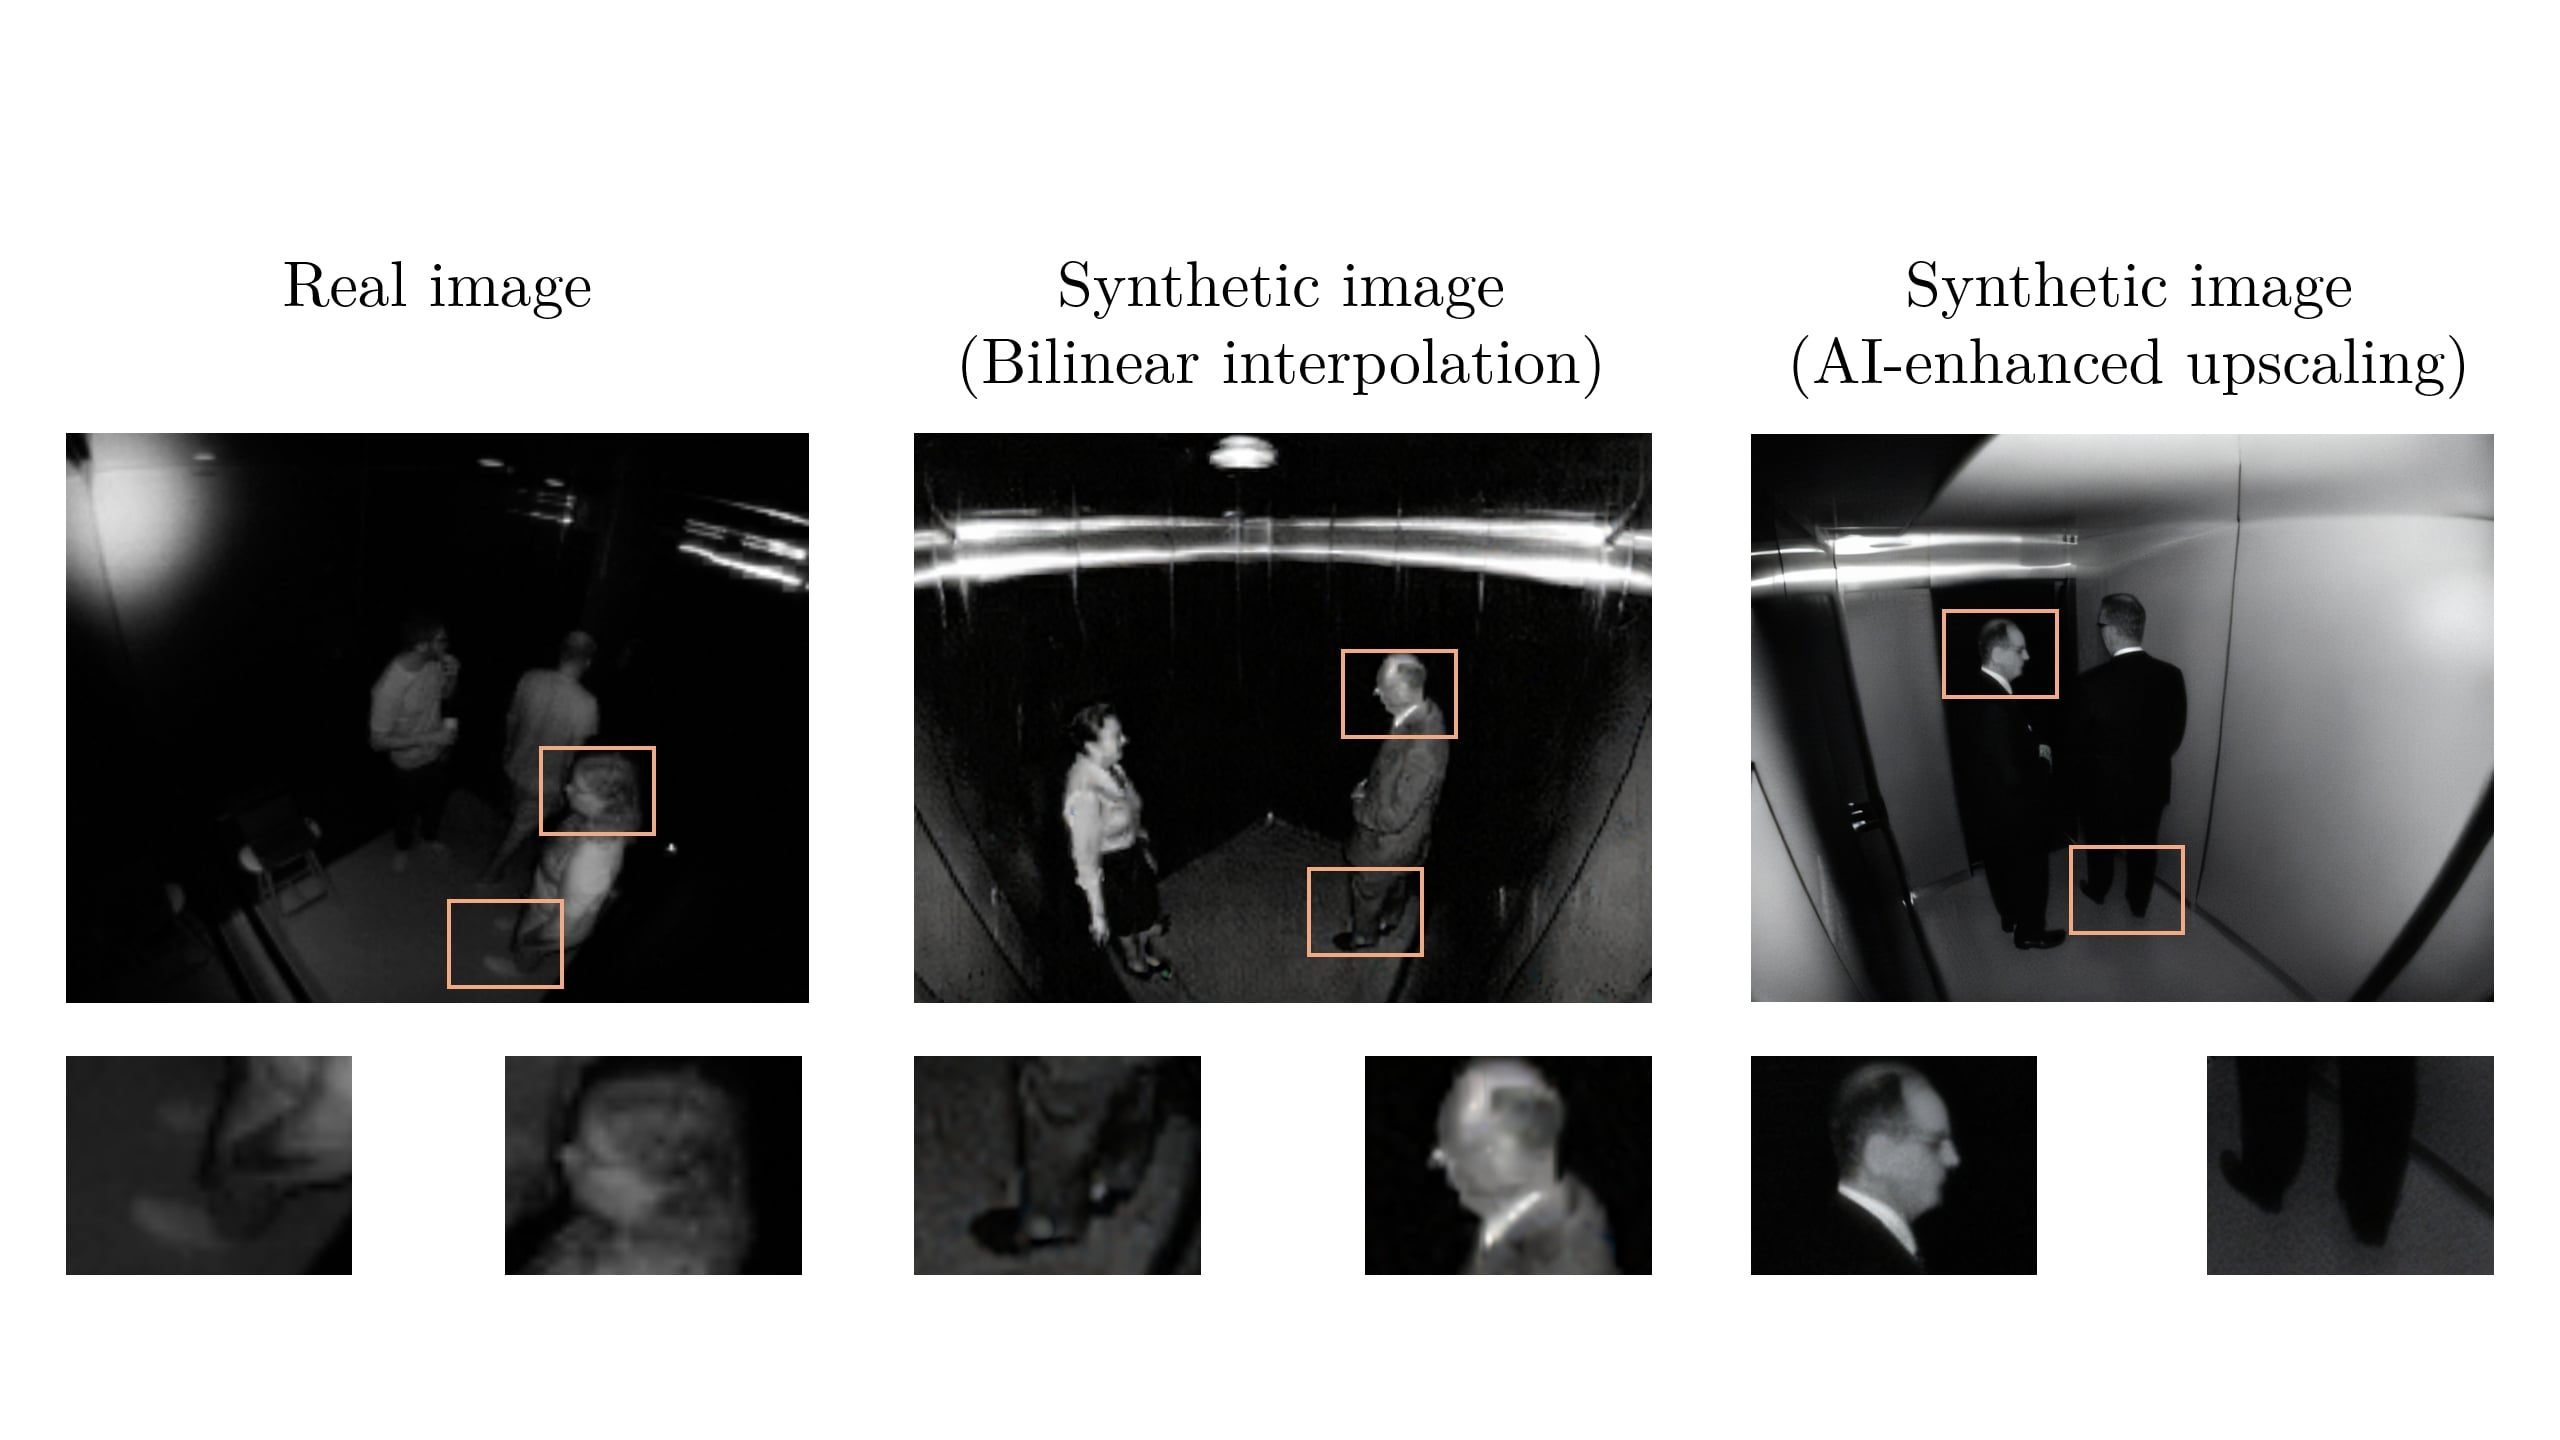
\includegraphics[width=1\textwidth]{images/methotologies/generation/dataset3.jpg}
    \caption{Real image and synthetic images generated using different upscaling methods for LoRA training. From left to right: (a) Real image, (b) Synthetic image using bilinear interpolation, and (c) Synthetic image using AI-enhanced upscaling.}
    \label{fig:upscaling-methdod}
\end{figure}

Synthetic images in Figure~\ref{fig:upscaling-methdod} were generated using identical LoRA configurations (same hyperparameters, image-caption pairs, and random seed), except that the training datasets used different upscaling methods. Visual inspection indicates that both methods can mimic the monochromatic characteristics of the original images. However, compared to the original dataset, images generated using bilinear interpolation appear to have rougher noise patterns, while those generated using Upscayl exhibit smoother textures. Without any quantitative evaluation, both approaches appear to be visually realistic enough for object detection model training.

The decision to use Upscayl in this work was primarily based on early experiments where captioning was unintentionally left out during LoRA training with the bilinear interpolation dataset, leading to less consistent generation performance. Since the focus of this work was to design a complete pipeline from scratch, it was decided to proceed with Upscayl as it produced sufficiently realistic results.

\subsection{Image Captioning}
Captions are textual descriptions that provide information about the content of an image. As discussed in Section~\ref{sec:conditioning}, the text encoder captures visual characteristics such as style, objects, and actions within a shared embedding space, making it possible to guide image generation. In LoRA training, even though only the weights of the U-Net are fine-tuned, the model remains conditioned on the outputs of the text encoder. Therefore, the information contained in captions indirectly guides the optimization of the U-Net weights. When a model is trained without captions, it still learns the features of the training dataset, but the resulting images exhibit limited flexibility and controllability in prompt-based image generation. This is the main motivation for using captions in training.

Since there was a lack of published research papers at the time of implementation, the primary guidelines for captioning were derived from the experience of the Stable Diffusion community \cite{followfoxai_impact_style_training_2023, civitai_flux_lora_2024, reddit_lora_captioning_2024,reddit_no_captions_lora_2024,reddit_adv_model_training_2023}. The main principle can be summarized as follows: \textit{"Features that we want to control later in image generation should be mentioned in the captions."}

Within the community, there are mainly used four different captioning strategies: no captions, natural language, tags, or a combination of both natural language and tags. Table~\ref{tab:captionexample} provides an example of captioning using both natural language and tags.


 \begin{table}[h]
        \caption{Example captioning of the bottom-right image from Figure~\ref{fig:people} using natural language and tags.}
    \label{tab:captionexample}
    \centering
    \begin{tabular}{|p{0.5\textwidth}|p{0.4\textwidth}|}
    \hline
         Natural language & Tags \\ \hline
          A group of three people walk together in the rain under umbrellas. They are wearing coats and carrying bags on their shoulders. In the background, there is a grassy area with a wooden bench and a brick building with an open vent. & three people, rain, umbrellas, coats, bags, grassy area, wooden bench, brick building, open vent \\ \hline
    \end{tabular}
\end{table}

Natural language captions provide contextual descriptions using full sentences, while tags describe content of the image through short keywords. In this work, a combination of both was used: natural language for elements requiring fine-grained control (e.g., describing clothing or actions of people), and tags for simpler attributes (e.g., presence of mirrors or lighting condition in the elevator). This approach increase caption diversity while remaining compact and providing good control over important features.\footnote{Some community guidelines also recommend using unique tags to activate specific features, such as new object types or one of the multiple styles from the training dataset. Unique tags are not presented in pretrained text encoder, and letters are sometimes replaced with numbers or special characters to ensure uniqueness. For example, a good unique tag for NIR images could be "N1r1m4g3" as it is not likely presented in pretrained text encoder. In this work, unique tags were not used for feature activation, as the LoRA was expected to learn the characteristics of NIR from the training images itself even without captions.}

For captioning, Taggui was used, as it allows fast captioning of multiple images simultaneously—for example, assigning shared tags to similar images. Taggui also includes an option to generate captions using the BLIP captioner, but it did not recognize content of NIR images correctly and was therefore not used. Figure~\ref{fig:captionexample} shows an example of an image–caption pair used in LoRA training.

\begin{figure}[!h]
    \centering
    \captionsetup[subfigure]{labelformat=empty}
    \subcaptionbox{Caption: \textit{ir-image, top-view perspective, dark elevator, a man is going out from an elevator carrying a box on his shoulder}}{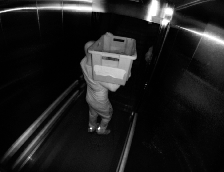
\includegraphics[width=1\textwidth]{images/methotologies/captions/4_bom_1_laatikon_kanssa_sitten_1_ilman_laatikkoa_frame66.png}} 
    \caption{Example image-caption pair used in LoRA training.}
   \label{fig:captionexample}
\end{figure}

In Section~\ref{sec:synthetic_data}, Figure~\ref{lora_weight_comparison} demonstrates how prompts were used in image generation, while Figure~\ref{wildcard_example} shows different scenarios generated by different prompts.


\subsection{LoRA Training}
For training the LoRA to fine-tune the SDXL base model, Kohya's GUI (also known as  \textit{kohya-ss}) was used. Tables \ref{tab:explanationloraparams} and \ref{tab:basicloraparams} summarize the most important hyperparameters and their values used in LoRA training process.


\begin{table}[h]
        \caption{Description of the most important hyperparameters for LoRA training \cite{kohya-lora-training}.}
    \label{tab:explanationloraparams}
    \centering
    \begin{tabular}{|p{0.2\textwidth}|p{0.7\textwidth}|}
    \hline
    \textbf{Hyperparameter} &  \textbf{Description}  \\ \hline
    \textbf{Learning Steps} & Total steps = number of images × repeats × epochs. Each step shows the model one image during training. \\ \hline
    \textbf{Repeats} & Number of times each image is shown per epoch. \\ \hline
    \textbf{Epochs} & Number of complete passes through the dataset (images and repeats). The model state can be saved after every $N$ epochs. \\ \hline
    \textbf{Batch Size} & Number of images processed simultaneously during training. Larger values increase VRAM usage and may slightly affect model performance. \\ \hline
    \textbf{Learning Rate (LR)} & Controls how much the weights are adjusted during optimization. Too high a value can cause the model to overfit, while too low a value can lead to underfitting. There are two types of LR in LoRA training: U-Net LR is for fine-tuning attention and other blocks in the U-Net, and Text Encoder LR determines the sensitivity to captions. The Text Encoder LR is usually lower than U-net LR, as it also affects the whole U-net. \\ \hline
    \textbf{Learning Rate Scheduler} & Adjusts the LR during training. Common schedulers are constant (constant LR), linear (decreasing LR linearly), and cosine (decreasing LR following a cosine curve).  \\ \hline
    \textbf{Optimizer} & Algorithm used to update network weights during training. Common optimizers are AdamW, AdamW8bit and Adafactor. \\ \hline
    \textbf{Max Resolution} & Sets the maximum training image resolution. Images exceeding this resolution are downscaled. \\ \hline
    \textbf{Buckets} & Groups training images of different sizes into resolution "buckets." Images are resized to standard size within the selected bucket resolution limits (if 'Don't upscale bucket resolution' is false). \\ \hline
    \textbf{Network Rank} & Defines the amount of information stored in the LoRA. A higher rank captures more detail but risks overfitting, while a lower rank has more consistency but less detail.  \\ \hline
    \textbf{Network Alpha} & Scaling factor for storing LoRA weights. The alpha/rank ratio affects the learning rate. \\ \hline
    \end{tabular}
    \end{table}

\begin{table}[h]
        \caption{Hyperparameter values used for LoRA training.}
    \label{tab:basicloraparams}
    \centering
    \begin{tabular}{|p{0.2\textwidth}|p{0.5\textwidth}|}
    \hline
    \textbf{Hyperparameter} & \textbf{Value} \\
    \hline
    Pretrained model & stabilityai/stable-diffusion-xl-base-1.0 \\
    \hline
    Save precision & BF16 \\
    \hline
    LoRA type & Standard \\
    \hline
    Train batch size & 1 \\
    \hline
    Epoch & 20 \\
    \hline
    Repeats & 20 \\
    \hline    
    LR Scheduler & Constant \\
    \hline
    Optimizer & Adafactor \\
    \hline
    Max resolution & 1536 x 1536 \\
    \hline
    Enable buckets & True \\
    \hline
    LR (U-Net and Text Encoder) & 0.0004 \\
    \hline
    Learning rate warmup steps & 0 \\
    \hline
    Network Rank & 32 \\
    \hline
    Network Alpha & 16 \\
    \hline
    \end{tabular}

\end{table}

The hyperparameter values in Table~\ref{tab:basicloraparams} were chosen based on experimentation and community experience. Training was performed using Stability AI's official SDXL checkpoint. The training dataset contained 31 captioned images, each repeated 20 times, resulting in 620 steps per epoch. Training ran for 20 epochs, and the LoRA weights were saved after every second epoch, allowing evaluation and comparison of LoRAs at different training stages. The batch size was set to 1 due to GPU memory limitations.

Adafactor was chosen as the optimizer because of its adaptive learning rate scaling and high memory efficiency \cite{shazeer2018adafactoradaptivelearningrates}. The maximum resolution was set high enough to ensure that all training images (1120 x 860) were below this threshold. Buckets were enabled to resize images to the nearest multiple of 64 while preserving the aspect ratio as closely as possible. As a result, training images were resized during training to 1088 x 832 pixels (aspect ratio $\approx$ 1.308) instead of 1120 x 860 (aspect ratio $\approx$ 1.302). For the network parameters, the rank and alpha were set correspondingly to 32 and 16. The resulting LoRA models reproduced the visual characteristics of the original NIR training data when applied to the SDXL base model, as shown in Figure~\ref{lora_weight_comparison}.

\subsection{Image Generation}
\label{sec:synthetic_data}
Image generation was performed using Stable Diffusion WebUI Forge, which is a platform built on top of Stable Diffusion WebUI (also known as \textit{AUTOMATIC1111}) \cite{stable-diffusion-webui}, designed to optimize resource management. The parameters used for the image generation are described in Table~\ref{tab:descimageparams}.

\begin{table}[h]
        \caption{Description of parameters used for image generation.}
    \label{tab:descimageparams}
    \centering
    \begin{tabular}{|p{0.2\textwidth}|p{0.7\textwidth}|}
    \hline
    \textbf{Parameter} & \textbf{Description} \\
    \hline
    Sampler & Defines the algorithm used for sampling (e.g., DDIM, PLMS, DPM++ 2M, Euler a). \\
    \hline
    Sampling step & Number of denoising iterations performed from random noise to the final image. \\
    \hline
    CFG scale & Classifier-Free Guidance (CFG) scale controls how strongly the text prompt will influences the diffusion process. There is a trade-off between diversity and accuracy: Higher value makes the sampling process follow the text prompt more strictly, while a lower value reduces the influence of the text prompt. \\
    \hline
    \end{tabular}
    \end{table}

Parameter sensitivity was analyzed by changing one parameter at a time while keeping the others fixed and repeating the process with several random seeds. This was also done for different LoRA models and strengths to determine which combination of LoRA model, strength, and parameter values produce the best results. An example comparing different LoRA strengths is shown in Figure~\ref{lora_weight_comparison}.

\begin{figure}[!h]
    \centering
    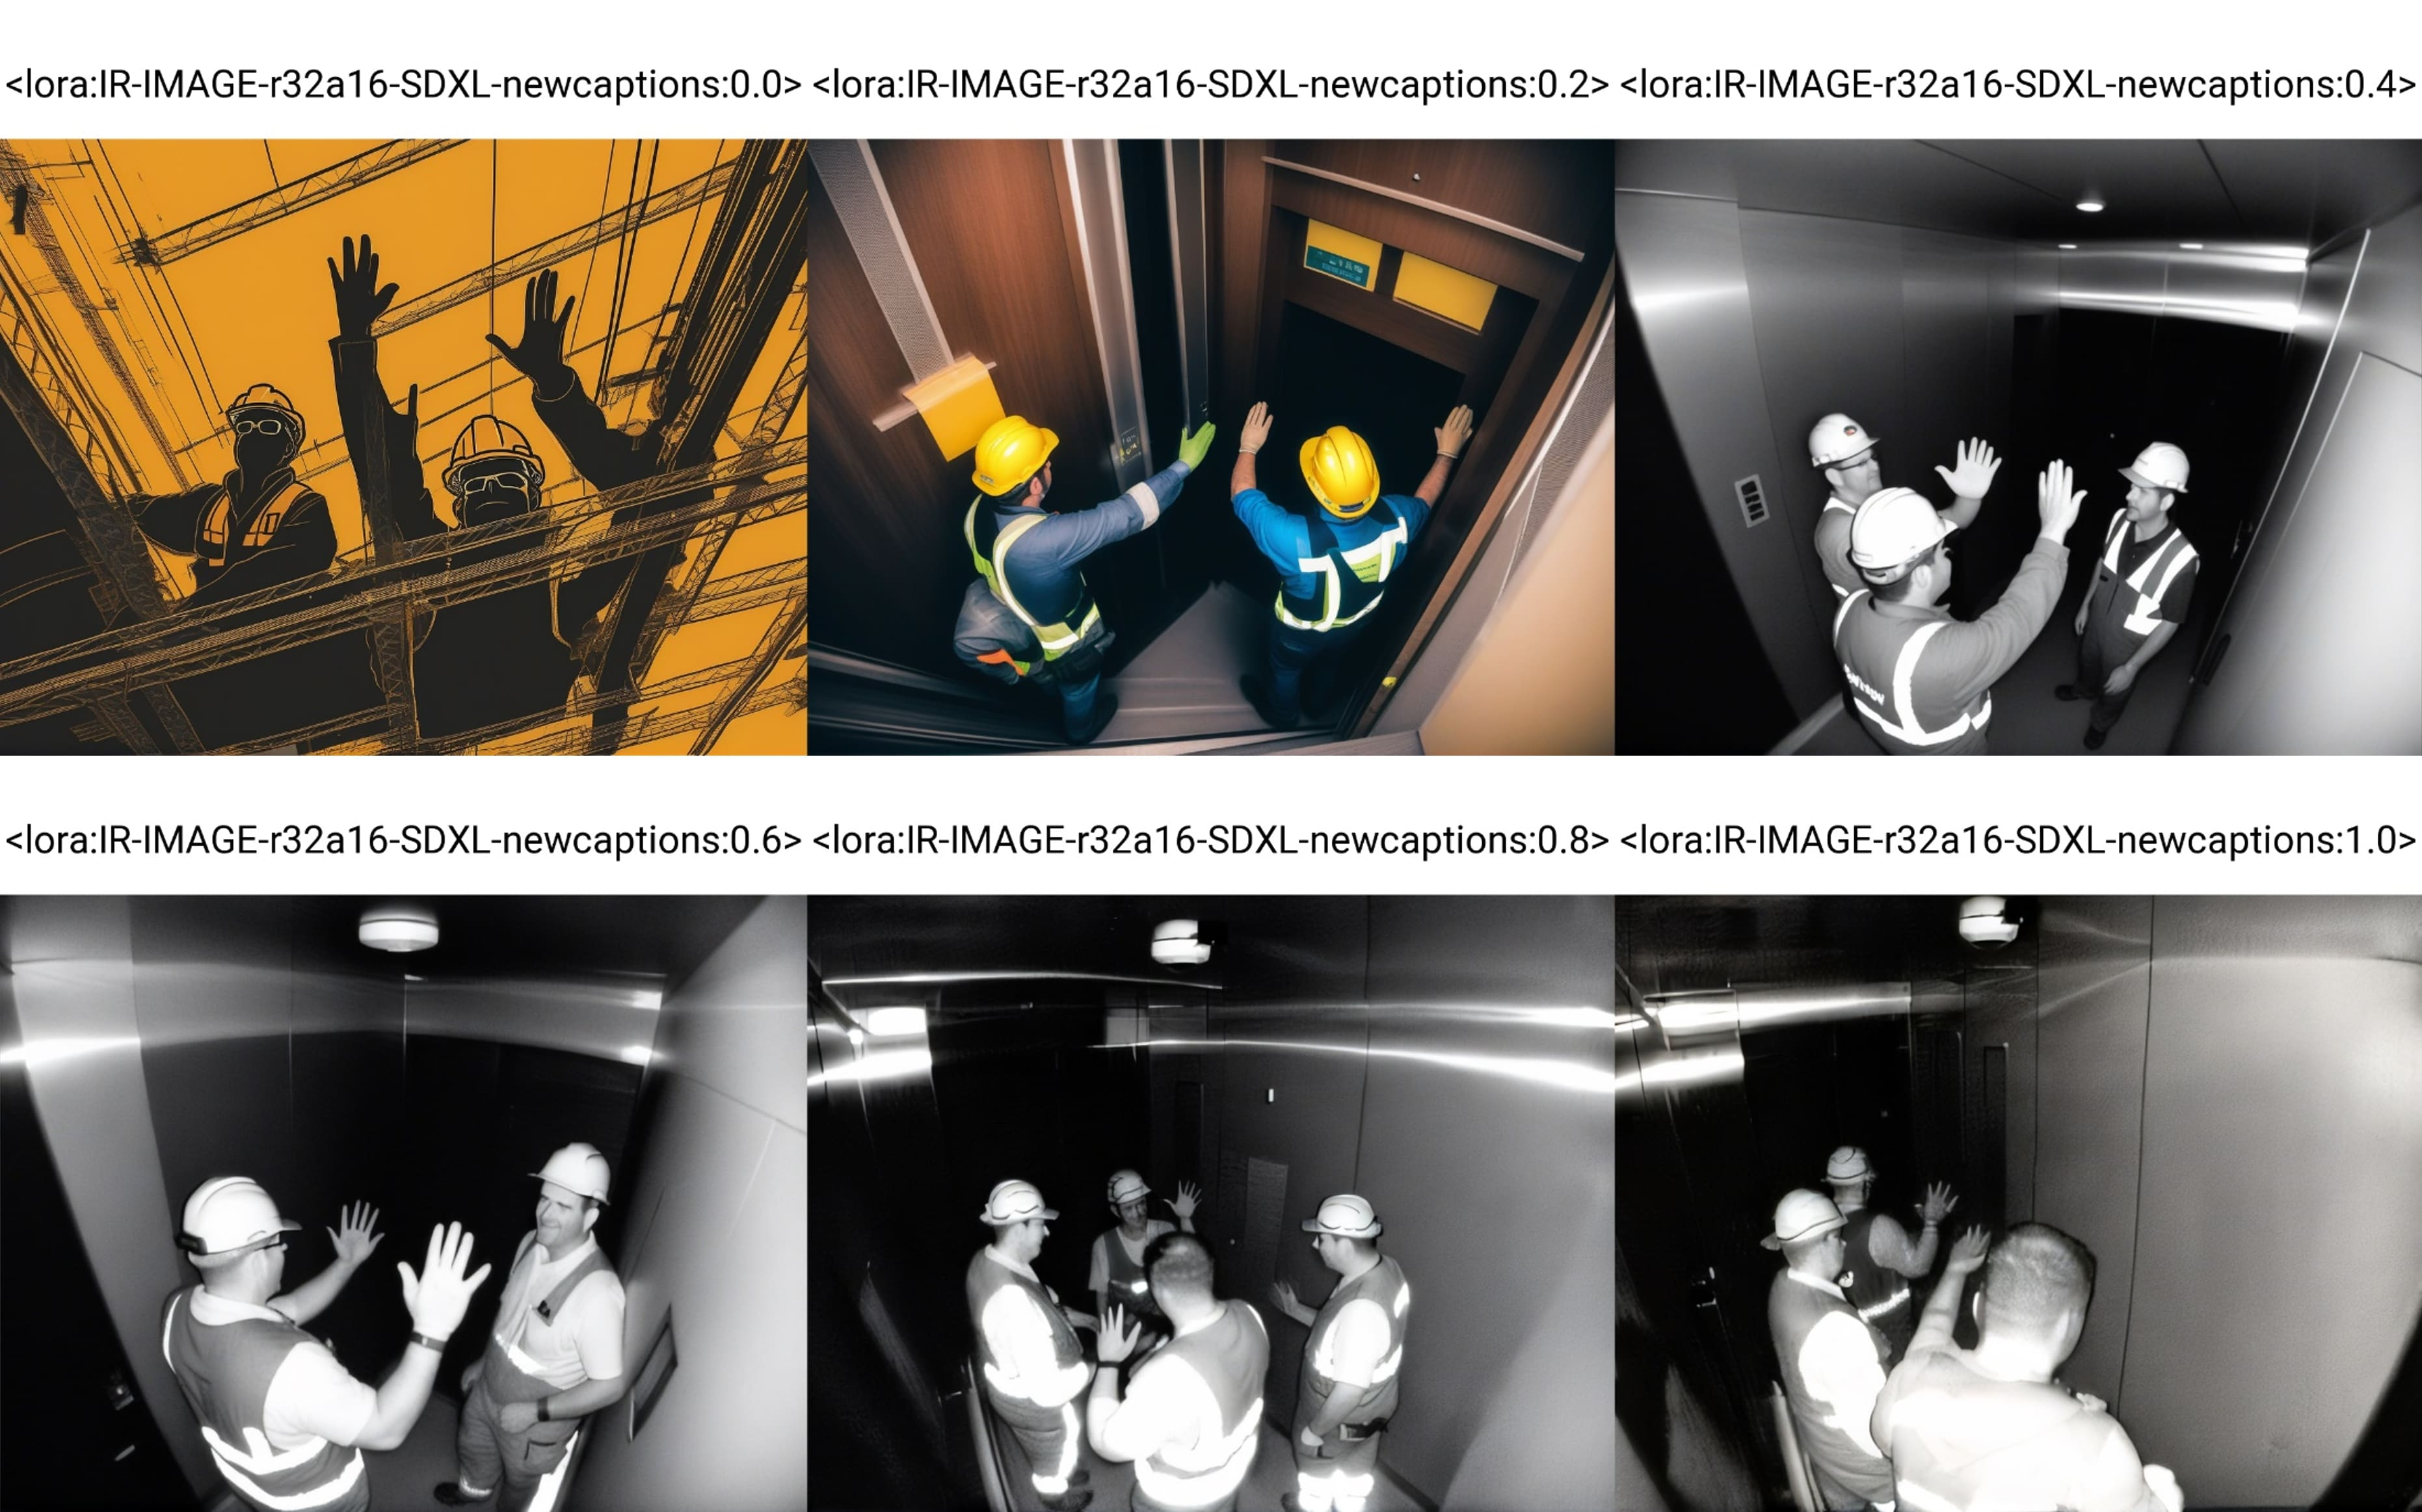
\includegraphics[width=1\textwidth]{images/methotologies/generation/Kuva2.jpg}
    \caption{Effect of different LoRA strengths on image generation using the following prompts:
    \textbf{Prompt:} \textit{ir-image, top-view perspective, two construction workers waving hands inside an elevator} \\
    \textbf{Negative prompt:} \textit{mutated body parts, disfigured, bad anatomy, deformed body features, metallic wall, mirror, (white clothes:1.2), beanie}}
   \label{lora_weight_comparison}
\end{figure}

From Figure~\ref{lora_weight_comparison}, it can be seen how different LoRA strengths affect image generation. The SDXL base model itself was unable to generate images inside an elevator, as described in the prompt. After applying a LoRA strength to 0.4, the similar characteristics captured from the NIR sensor started to appear, although images still appeared more defined and less noisy compared to the training images. Strengths between 0.6 and 0.8 provided a good balance between diversity and similarity. Beyond a strength of 0.8, generated images began to overfit, occasionally reproducing recognizable individuals from the training dataset. Based on these observations, a LoRA strength of 0.7 was selected for image generation. Similar examples for Sampler, Sampling step, and CFG scale are illustrated in Appendix~\ref{ch:appendix_image_generation}.

Based on these experiments, the parameters used for image generation are summarized in Table~\ref{tab:imagegen_params}.

\begin{table}[h]
        \caption{Values of the parameters used for image generation.}
    \label{tab:imagegen_params}
    \centering
    \begin{tabular}{|p{0.2\textwidth}|p{0.7\textwidth}|}
    \hline
    \textbf{Parameter} & \textbf{Value} \\
    \hline
    Height and width & 1088 x 832 \\
    \hline
    Sampler & Euler a \\
    \hline
    Sampling step & 20 \\
    \hline
    CFG scale & 7 \\
    \hline
    \end{tabular}
\end{table}

To generate a diverse set of synthetic images, the wildcard extension tool was used to randomize prompts. Wildcards allow defining collections of words under wildcard variable that are randomly selected during image generation. For example, a custom wildcard variable \texttt{\_\_amount\_of\_people\_\_} could randomly be replaced by "one", "two", "three", "a few" ,"many" or "large group of". In this work, wildcards were used to control various attributes such as environment, action, and number of people, as shown in Figure~\ref{wildcard_example}.

\begin{figure}[!h]
    \centering
    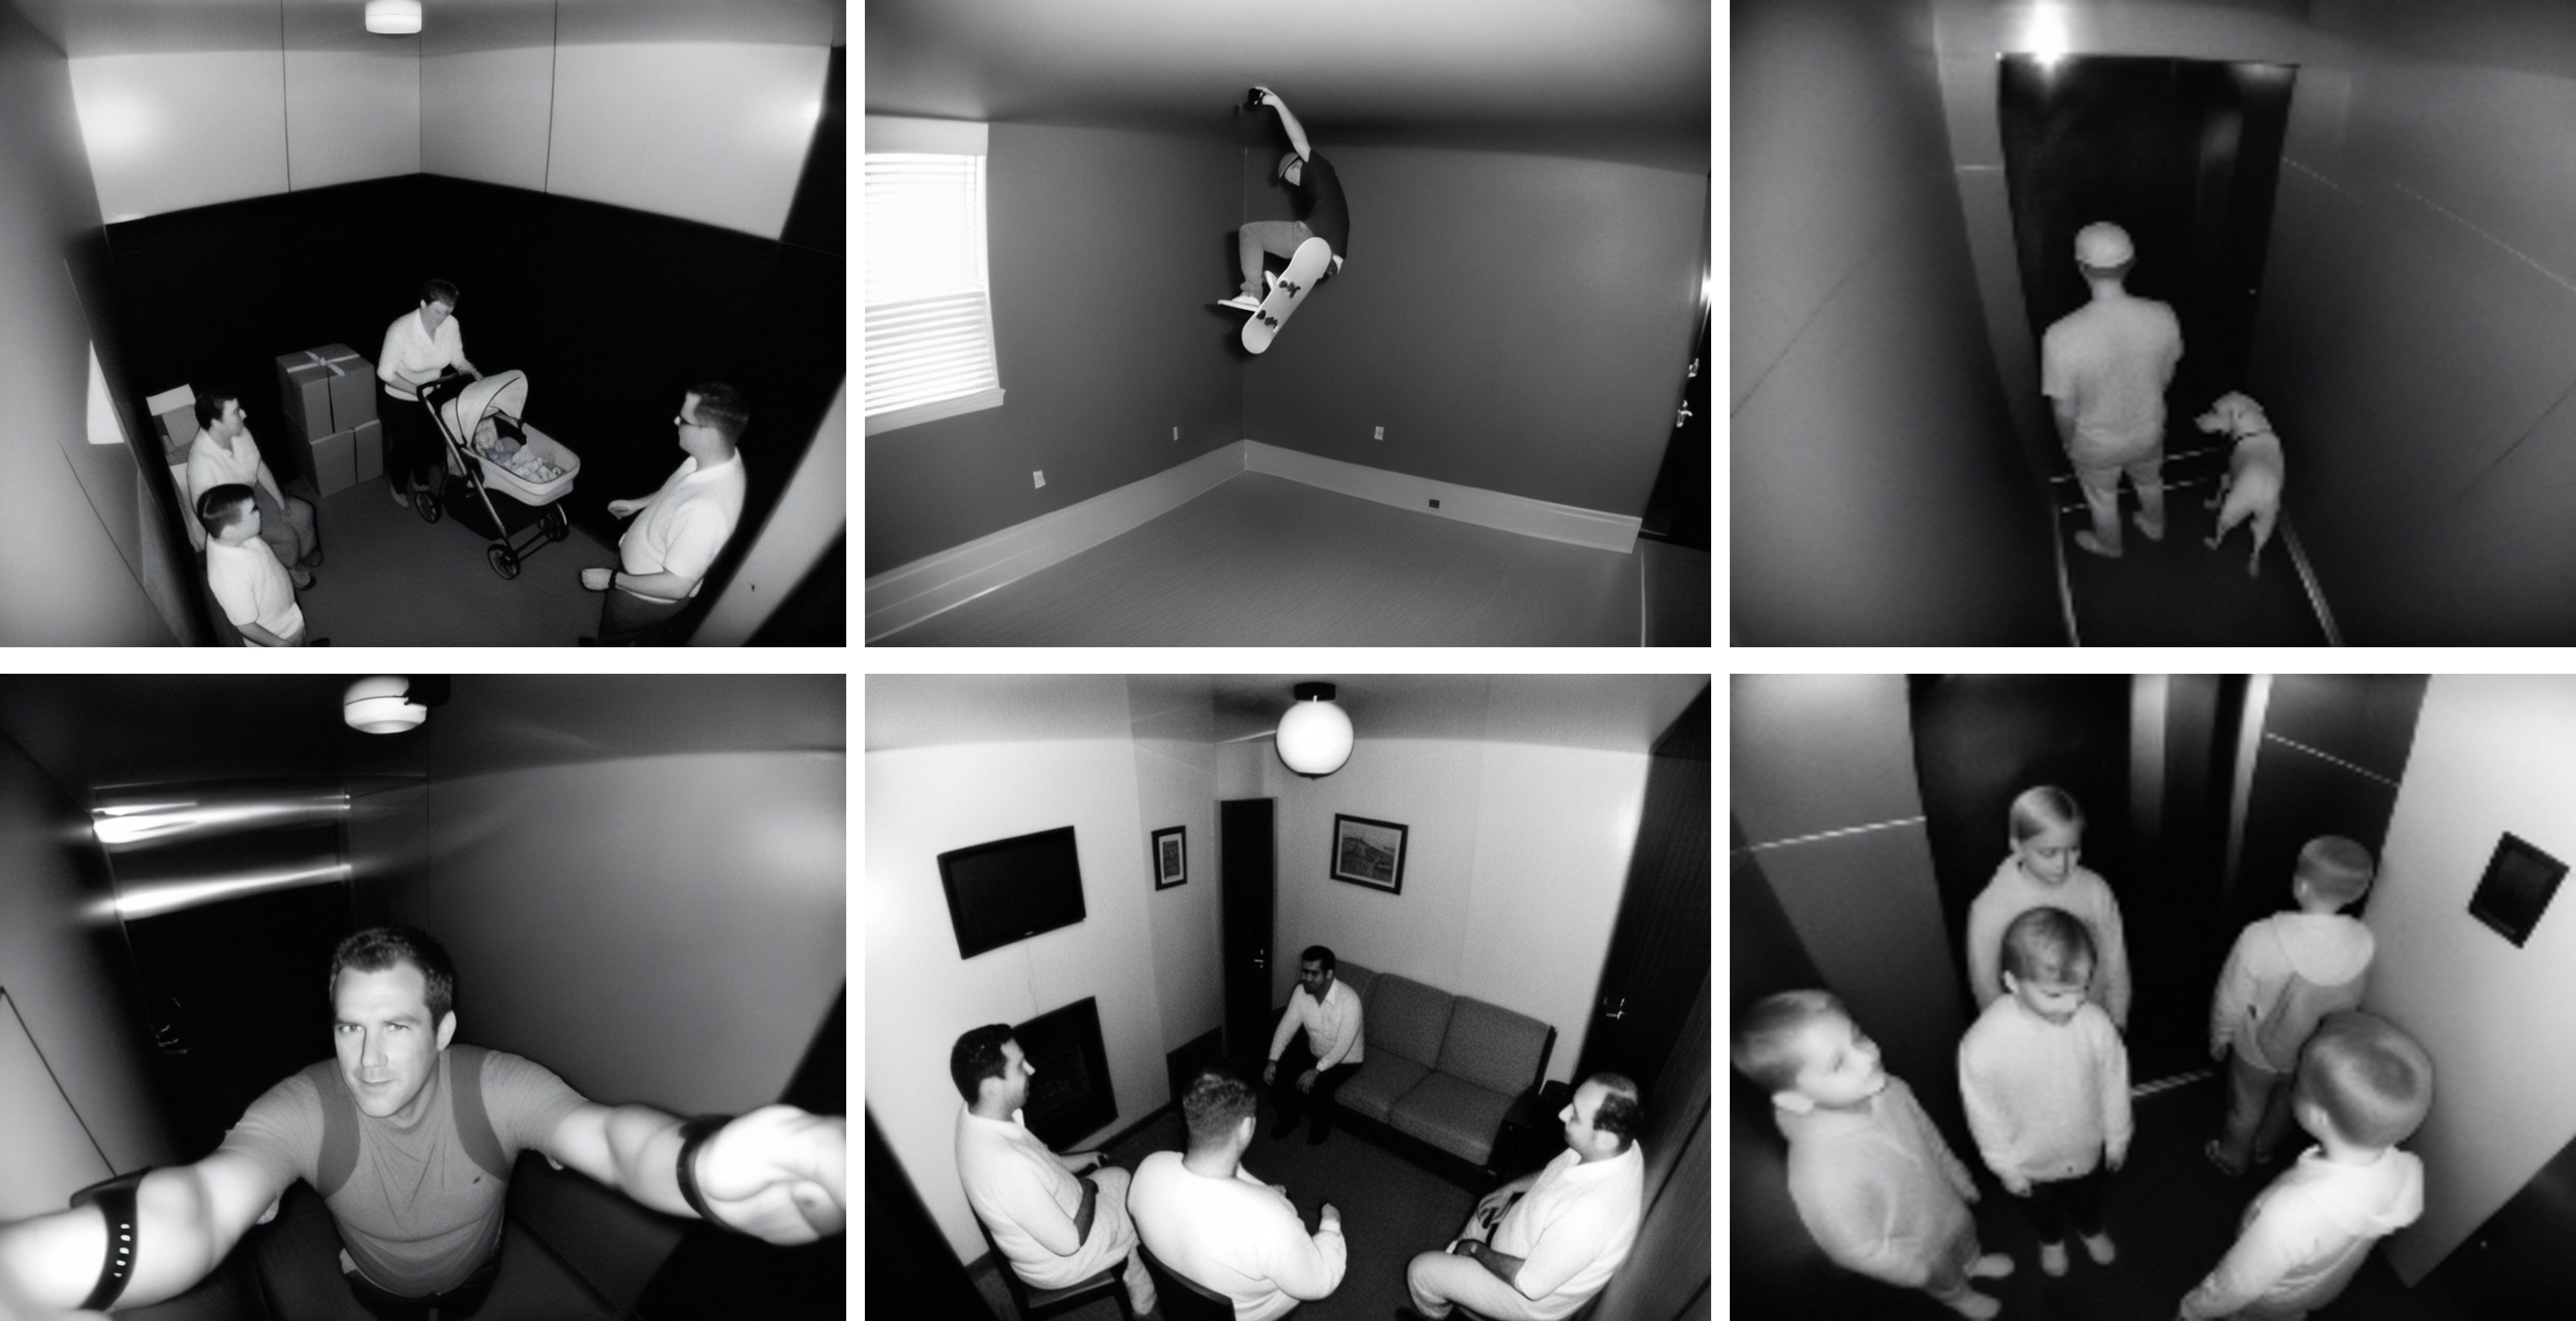
\includegraphics[width=1\textwidth]{images/methotologies/generation/Kuva3.jpg}
    \caption{Example of images generated using wildcards in prompts.}
   \label{wildcard_example}
\end{figure}

A total of over 4000 images were generated, after which images with visible color artifacts, overrepresented attributes or unrealistic distortions were removed. From cleaned synthetic dataset, 2500 images remained for training object detection models. The average generation time with the chosen parameters was approximately 6 seconds per image using an RTX 3080 10GB GPU.

\section{Object Detection Model Training}
\label{sec:object_detection_training}

The cleaned synthetic dataset of 2500 images was resized to 224 x 172 pixels to match the resolution of the original NIR sensor images. Both synthetic and real images were annotated using Darkmark, a GUI tool for annotating images, in which people were labeled by drawing bounding boxes around them. To reduce manual labour, a pretrained YOLOv8l model was used to automatically pre-annotate the dataset. This approach was able to correctly detect some people and provided a good starting point for manual annotation, although many cases were missed. As the annotation process progressed, a YOLOv8l model was fine-tuned using already annotated images to improve detection accuracy and assist even better in pre-annotating the remaining synthetic images.

To evaluate how synthetic images affect fine-tuned model performance, 23 separate models were trained using different combinations of real and synthetic images. The real image subsets included 0, 200, 400, and 568 images, while the synthetic image subsets included 0, 500, 1000, 1500, 2000, and 2500 images; each larger subset contained all images from the previous, smaller subset. This resulted in 24 possible combinations, with the combination of 0 real and 0 synthetic images representing the base model without any fine-tuning.  For validation, 284 real images were used for all combinations.

For training, a pretrained YOLOv8n model was fine-tuned using the Ultralytics Python library. Hyperparameters were selected based on \cite{xin2024dartautomatedendtoendobject} and are presented in Table~\ref{tab:yolo_hyperparameters}. Additionally, the first 10 layers of the model were frozen, as the base model was capable of detecting people.

\begin{table}[h]
        \caption{Hyperparameters used for YOLOv8n fine-tuning.}
    \label{tab:yolo_hyperparameters}
    \centering
    \begin{tabular}{|p{0.4\textwidth}|p{0.2\textwidth}|}
    \hline
    \textbf{Hyperparameter} & \textbf{Value} \\
    \hline
    Epochs & 60 \\
    \hline
    Optimizer & AdamW \\
    \hline
    Momentum & 0.9 \\
    \hline
    Image size & 640 \\
    \hline
    Initial learning rate & 0.0027 \\
    \hline
    Learning rate factor & 0.5 \\
    \hline
    Batch size & 64 \\
    \hline
    Cosine learning rate & True \\
    \hline
    Warmup epochs & 4 \\
    \hline
    Single class & True \\
    \hline
    Freeze layers & 10 \\
    \hline
    Seed & 0 \\
    \hline
    \end{tabular}
\end{table}

The detection settings and the measured evaluation metrics of the fine-tuned models are presented in Chapter~\ref{ch:results}.




